\chapter{Determination of Exchange Stiffness of STT-MRAM devices with broken symmetry}

We have developed one of the world most sensitive spin-torque ferromagnetic resonance(ST-FMR)\cite{FieldMod} and we would like to accurately determine the exchange stiffness of the Magnetic Tunnel Junctions. The exchange interaction is essential since it determines the energy scale of two adjacent spins in the magnetic materials. Its value also affect the formation of magnetic structures such as domain walls and vortices. Therefore it is important for both fundamental scientific interest and technology development to measure the exchange stiffness from simple structures such as monolayer superlattices and thin films to complex systems such as the Magnetic Tunnel Junctions(MTJ). It has been demonstrated that the exchange stiffness in in-plane magnetized MTJs can be estimated by measuring the thermal stability factor and fit of model based on nucleation-type magnetization reversal\cite{thermalEx} and by modelling from microwave noise spectroscopy\cite{noiseEx}. It has also been showed that MTJs with perpendicular magnetic anisotropy can be utilized by characterizing the spin wave dispersion to determine the exchange stiffness\cite{chris}\cite{PMAEX}. However previous studies involving MTJs are focused on nominal circular devices and only rely on the mode spacings between first higher order modes and quasi-uniform modes. However the symmetry breaking in the nominal circular devices\cite{excitation2},which is often inevitable during the fabrication of the STT-MRAM devices, has altered the spin wave modes. In this chapter we would like to perform a comprehensive review of determining the exchange stiffness on both nominal circular devices and stadium shaped devices with different lateral dimensions.

\section{Measurement of ST-FMR on nominal circular devices}

The experimental set-up is based on Fig.\ref{fig:FMR_set_up} where we employ the field modulation technique to improve the signal-to-noise ratio. The STT-MRAM devices we measured are CoFeB based Magnetic Tunnel Junctions. We are mainly focused on the field-domain ST-FMR which sweeps the magnetic field at fixed constant driven frequency. We find that the field-domain measurement is usually faster and yields better signal compared with frequency-domain. 

\begin{figure}[!ht]
\centering
\subfigure{\label{fig:C07MR}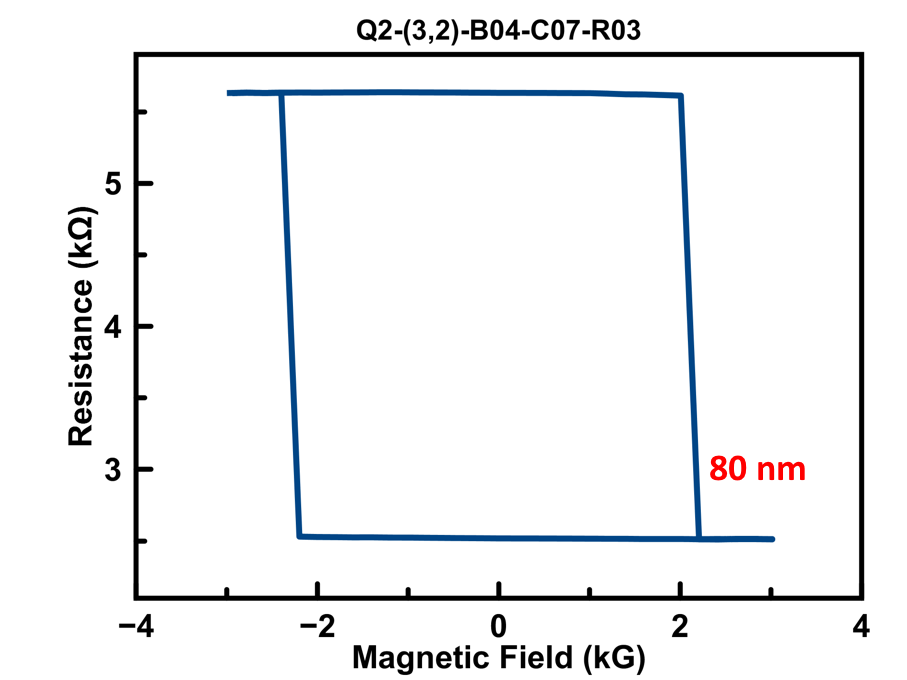
\includegraphics[width=75mm]{fig/2018/C07MR}}
\subfigure{\label{fig:C07FH}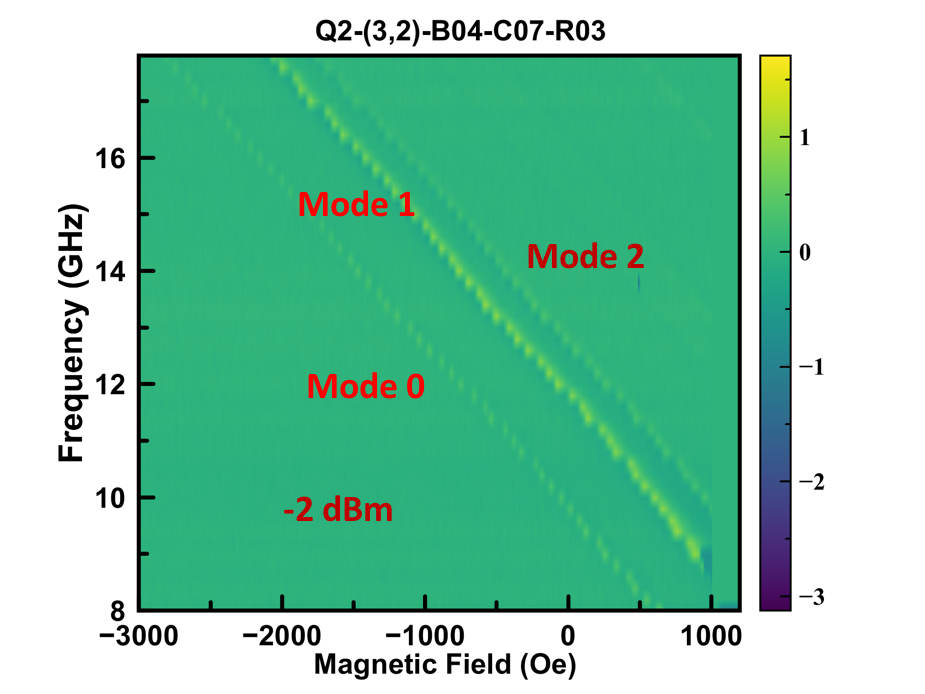
\includegraphics[width=75mm]{fig/2018/C07FH}}
\caption{(a) Example magnetoresistance of one 80 nm MTJ device (b) 2D contour plot of the ST-FMR signal of this device with -2 dBm power applied at the AP state  }
\end{figure}

We start with nominal circular devices with diameter ranging from 70 nm to 210 nm. Fig.\ref{fig:C07MR} shows an example magnetoresistance of 80 nm MTJ device. This specific device has resistance of 2511 Ohms at the parallel state and 5631 Ohms at the anti-parallel state. The coercive field is about 2100 Oe. Fig.\ref{fig:C07FH} shows the 2D contour plot of the ST-FMR signal of this device with -2 dBm power applied at the AP state. From the 2D contour plot we can mainly identify three of the spin wave modes, each of them labelled on the plot. The lowest mode(Mode 0) is the quasi-uniform main mode of the free layer in the MTJs. Mode 1 and Mode 2 is the split first higher order mode(we will discuss the mode profile in the next section).

\begin{figure}[!ht]
  \centering
  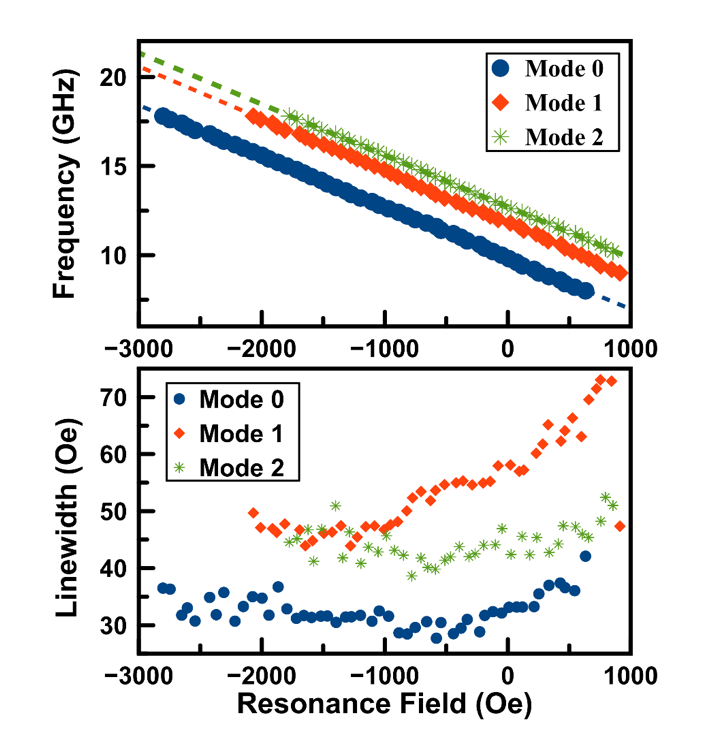
\includegraphics[width=0.6\textwidth]{fig/2018/C07fit}
   \caption{Top: the frequency versus resonance field for three lowest modes. Bottom: the HWHM linewidth versus resonance field for all the three modes.  }
  \label{fig:07fit}
\end{figure}

Fig.\ref{fig:07fit} summarizes the mode fitting result for all the three modes we excited from this 80 nm device. The top panel shows the frequency versus resonance field for three lowest modes. We can see a linear relation between the driven frequency and the resonance field as predicted by the Kittel equation. The main mode at zero field is 9.83 GHz and the effective anisotropy field Hk around 3.4 kG. The bottom panel shows the HWHM linewidth versus resonance field for all the three modes. Quite surprisingly, linewidth does not have a strong field dependence from -3000 Oe to 500 Oe (and frequency change by nearly a factor of 4). In theory, the linewidth in the field domain should be given by
\begin{equation}
	\Delta H = \alpha  \frac{\omega}{\gamma} + \Delta H_0
\end{equation}
Here, $\Delta H$ is the field-domain HWHM linewidth. $\omega = 2 \pi f$ is the angular frequency. $\gamma / 2 \pi$ is the gyromagnetic ratio. Firstly, this non-linear relation reveals that the fundamental understanding of the large non-Gilbert contribution to the damping is lacking. Secondly, we find that the linewidth for this device is relatively small (around 35 Oe). If we use the zero-field linewidth as upper bound, we have an estimation of Gilbert damping around 0.01. 


So far we have demonstrated that by performing the ST-FMR measurements, we can determine the "resonance frequency" at zero magnetic field for all the modes excited in the experiment. The frequency of the main mode can be used to determine the effective anisotropy field and the mode spacings between the main mode and the higher order mode is related with the exchange stiffness of the free layer. Before we move to the exchange stiffness, let us first discuss the original of the ST-FMR signal in this perpendicular magnetized MTJs.




\clearpage


\section{Study of signal amplitude of ST-FMR signal}

While we have not discussed the origin of the ST-FMR signal in the perpendicular magnetized MTJs with magnetic field applied in the easy axis, the exact source of the signal is not very clear. In fact, in a ideal circular device with rotation symmetry, such arrangement should yield no DC self rectification since the spin transfer torque is zero with free layer pinned in the perpendicular direction. However, we can still detect a measurable signal out of this set-up. It is argued that there are local misalignments between the uniaxial anisotropy and applied magnetic field due to shape distortion\cite{chris}. It is also possible that the non-uniformity of spin-transfer torque from the tunnel current across the free layer and non-uniform  tunnel magnetoresistance (TMR) should contribute to the ST-FMR signal. Previous work has been done to quantitatively measure the spin-transfer-torque in the ST-FMR signal\cite{Sankey2008}\cite{Kubota2007} for the MTJs with in-plane easy axis. However, in our field-modulated ST-FMR set-up, such experiments are not accessible since we are actually measuring the field derivatives of the real signal. Nevertheless, we still would like to qualitatively measure the signal amplitude of our ST-FMR data and try to gain some knowledge out of it.


\begin{figure}[!ht]
\centering
\subfigure{\label{fig:C10MR}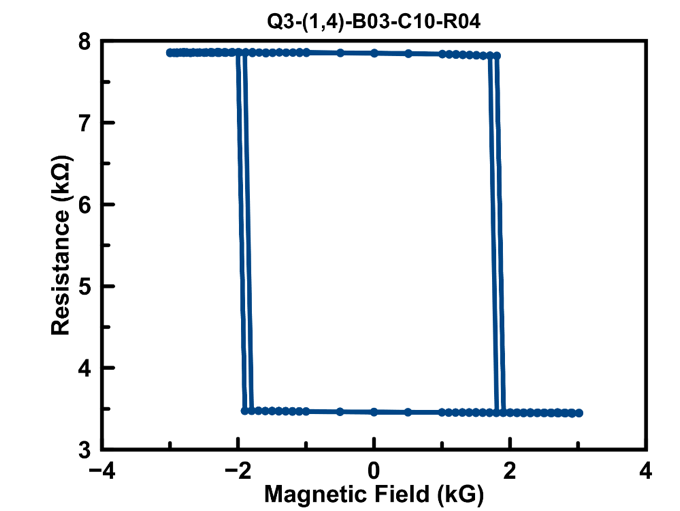
\includegraphics[width=50mm]{fig/2018/C10MR}}
\subfigure{\label{fig:C10RDC}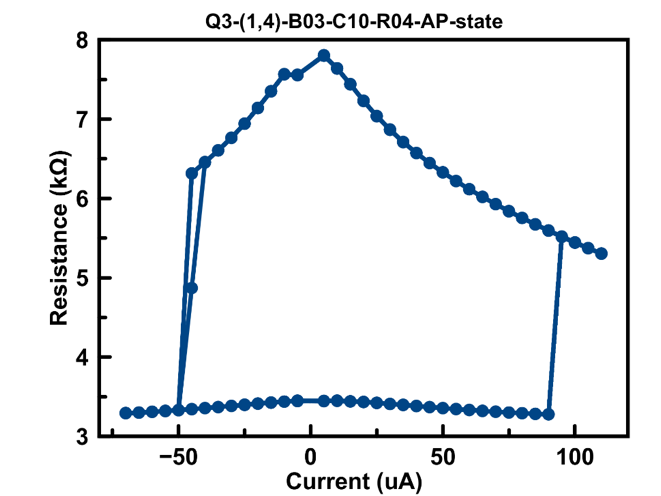
\includegraphics[width=50mm]{fig/2018/C10RDC}}
\subfigure{\label{fig:C102D}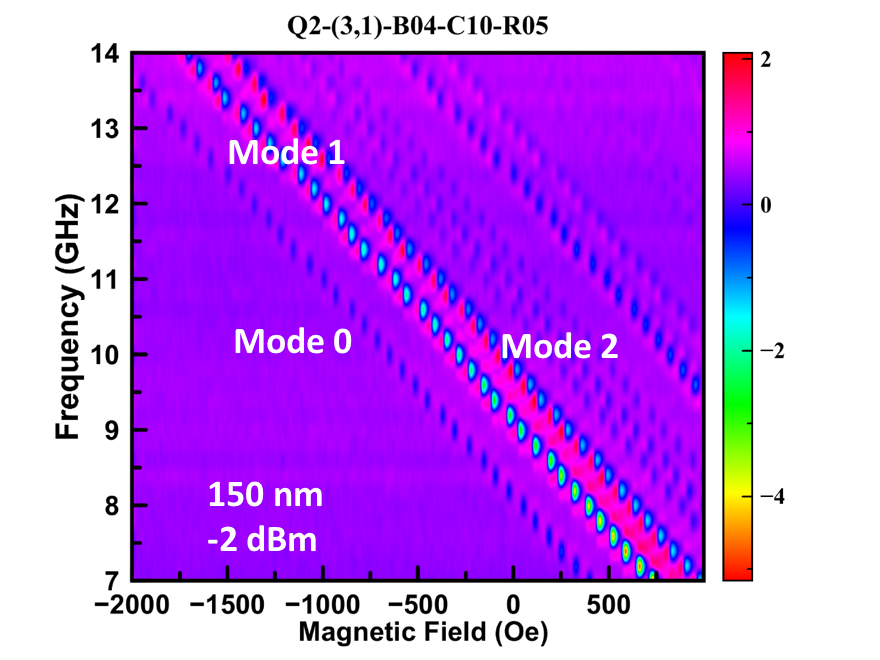
\includegraphics[width=50mm]{fig/2018/C102D}}
\caption{(a) Example magnetoresistance of one 60 nm * 80 nm stadium-shaped MTJ device. (b) The resistance versus current loop, with AP state switching to P state at negative dc current and vice versa. (c) 2D contour plot of the ST-FMR signal of this device with -2 dBm power applied at the AP state }
\end{figure}

The device employed in this study has a stadium shape with lateral dimensions 60 nm * 80 nm. Fig.\ref{fig:C10MR} shows the magnetoresistance of this device, which has resistance of 3445 Ohms at the parallel state and 7800 Ohms at the anti-parallel state. The coercive field is about 1850 Oe. Fig.\ref{fig:C10DC} shows the resistance versus current loop. The negative(positive) current is the anti-damping polarity for AP to P(P to AP)state. This demonstrate the effect of spin-transfer-torque switching. Fig.\ref{fig:C102D} shows the 2D contour plot of the ST-FMR signal of this device with -1 dBm power applied at the AP state. Again we can mainly identify three of the spin wave modes. 

\begin{figure}[!ht]
\centering
\subfigure{\label{fig:C10FH}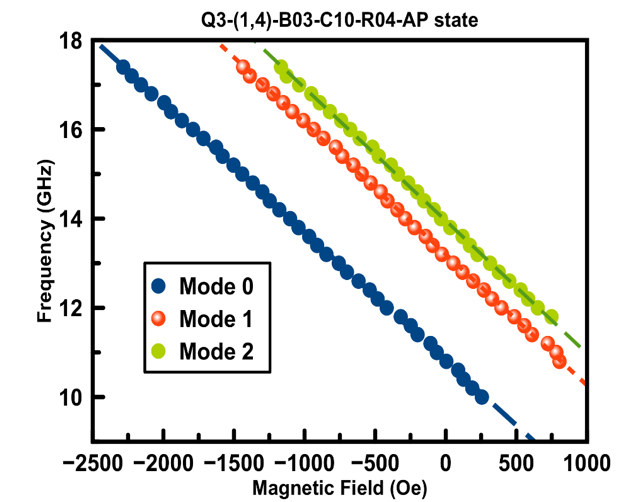
\includegraphics[width=50mm]{fig/2018/C10fit}}
\subfigure{\label{fig:C10signal}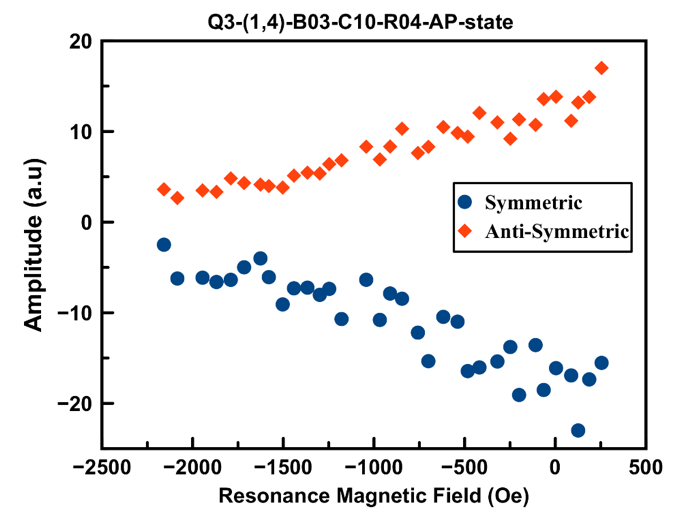
\includegraphics[width=50mm]{fig/2018/C10signal}}
\subfigure{\label{fig:C10ratio}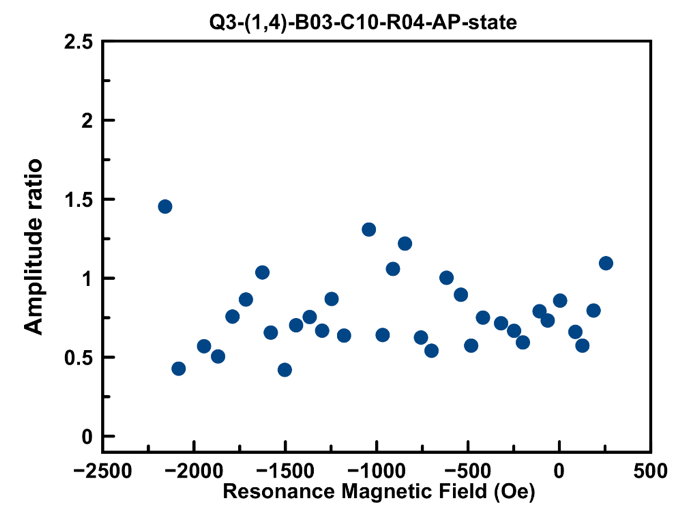
\includegraphics[width=50mm]{fig/2018/C10ratio}}
\caption{(a) The resonance field fitting result for all the three modes. (b) The ST-FMR signal (symmetric and anti-symmetric component) plot versus resonance field. (c) The ratio of two components versus resonance magnetic field. }
\end{figure}

Fig.\ref{fig:C10FH} summarizes the mode fitting result for all the three modes we excited from this stadium shape device. The linear relation is reproduced as expected. The main mode at zero field is 10.81 GHz and the effective anisotropy field Hk around 3.7 kG. Fig.\ref{fig:C10signal} shows the ST-FMR signal (symmetric and anti-symmetric component) plot versus resonance field. The amplitude is larger at small field and smaller at negative large magnetic field. This is due to magnetic susceptibility as expected. As we can see from Fig.\ref{fig:C10MR} that the MTJ at the AP state aligns better with the external negative magnetic field, which gives smaller ST-FMR amplitude. Fig.\ref{fig:C10ratio} shows the ratio of two components versus resonance magnetic field. And we see that the ratio remain relatively unchanged over the resonance field. The ratio of this two components is related with different signal mechanism which will be discussed later.

\begin{figure}[!ht]
\centering
\subfigure{\label{fig:C10power}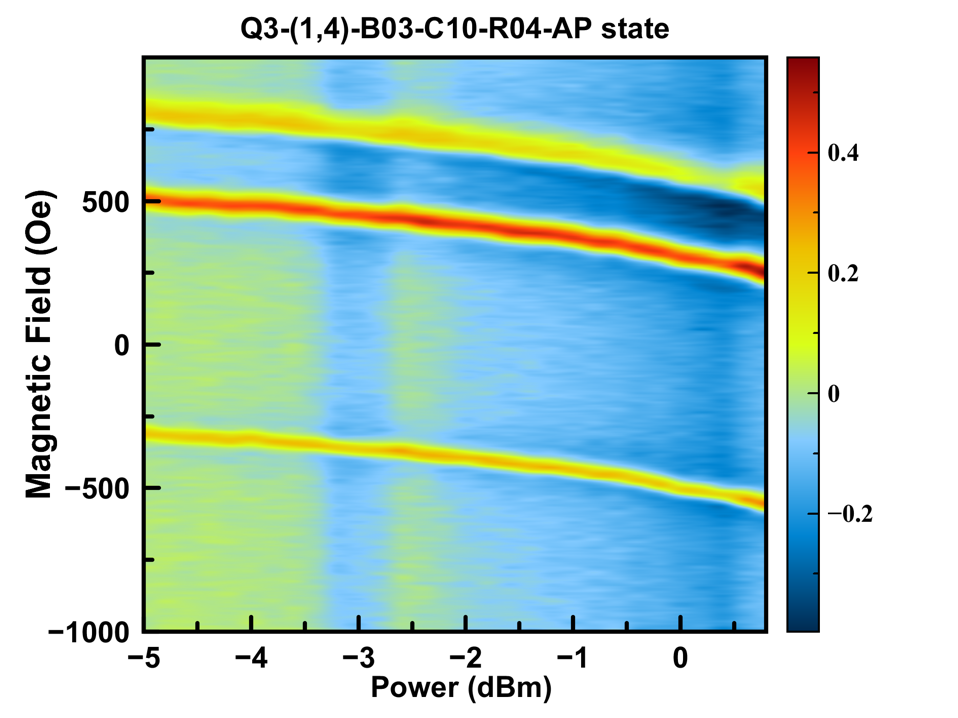
\includegraphics[width=75mm]{fig/2018/C10power}}
\subfigure{\label{fig:C10poweramp}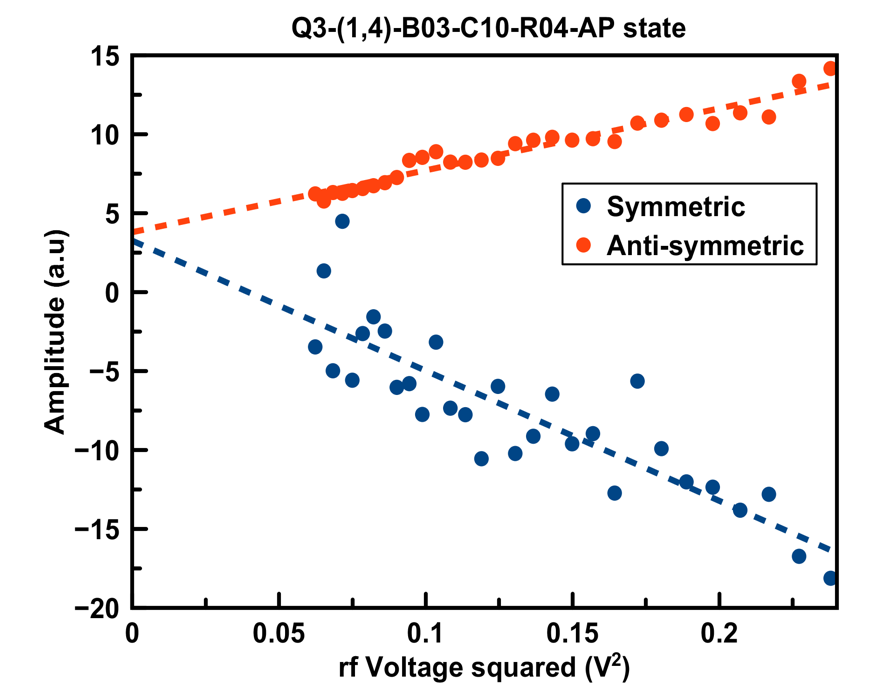
\includegraphics[width=75mm]{fig/2018/C10powersignal}}
\caption{(a) The power-dependent ST-FMR field sweep spectrum at AP state with 12 GHz. (b) The amplitude versus the square of rf voltage.}
\end{figure}

The applied power determines the rf voltage across the MTJs. Fig.\ref{fig:C10power} shows the power-dependent ST-FMR field sweep spectrum at AP state with 12 GHz. We can then plot the amplitude versus the square of rf voltage as shown in Fig.\ref{fig:C10poweramp}. The good linear fit indicating the ST-FMR signal mainly arises from rectification \cite{photovoltage1}. As the rf voltage approaches zero, both symmetric and anti-symmetric components goes to zero at a similar value. In fact, if we apply zero dc bias into the MTJ, this limit will go to zero at zero rf voltage. Thus we can confirm there is also a non-zero contribution from the photo-resistance effect\cite{photovoltage2}.


\begin{figure}[!ht]
\centering
\subfigure{\label{fig:C10powerfit}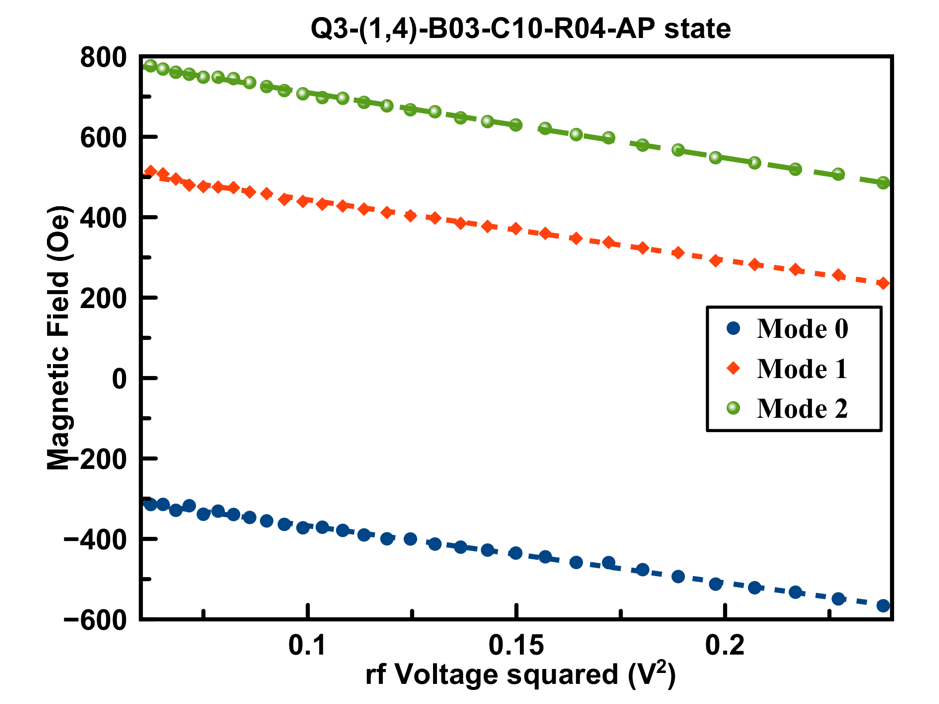
\includegraphics[width=75mm]{fig/2018/C10powerFH}}
\subfigure{\label{fig:C10powerLW}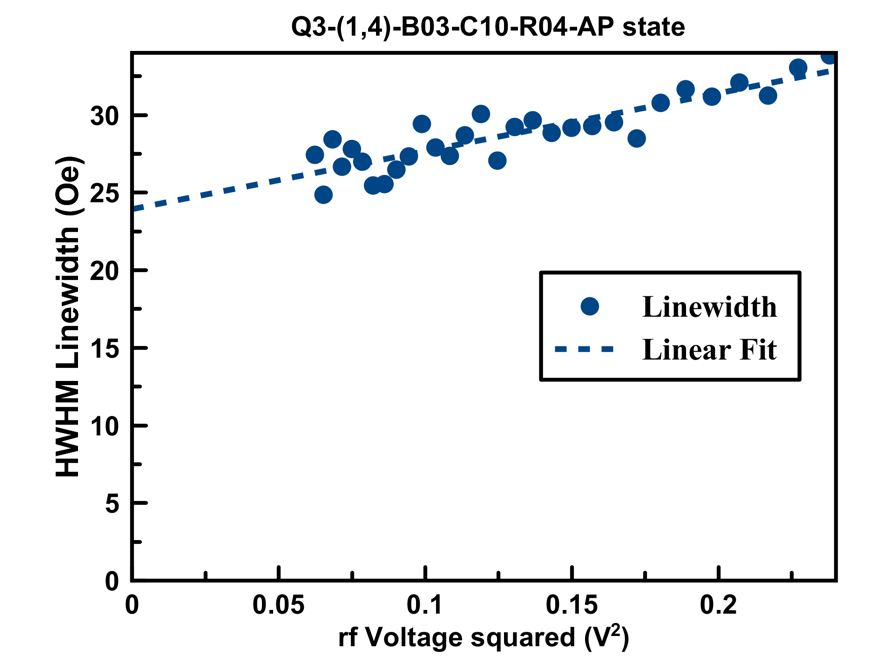
\includegraphics[width=75mm]{fig/2018/C10powerLW}}
\caption{(a) The resonance Field versus rf voltage squared  for all the modes at 12 GHz. (b) The Mode 0 HWHM linewidth versus rf voltage squared.}
\end{figure}

Fig.\ref{fig:C10powerfit} shows the resonance Field versus rf voltage squared  for all the modes at 12 GHz and Fig.\ref{fig:C10powerLW} shows the Mode 0 HWHM linewidth versus rf voltage squared. The linewidth shows a linear dependence with zero rf voltage linewidth around 23 Oe. The linear relation of both resonance field and linewidth ensures that we keep the ST-FMR measurement at the linear region where there is no non-linear broadening of the signal.
 
\begin{figure}[!ht]
\centering
\subfigure{\label{fig:C10DC}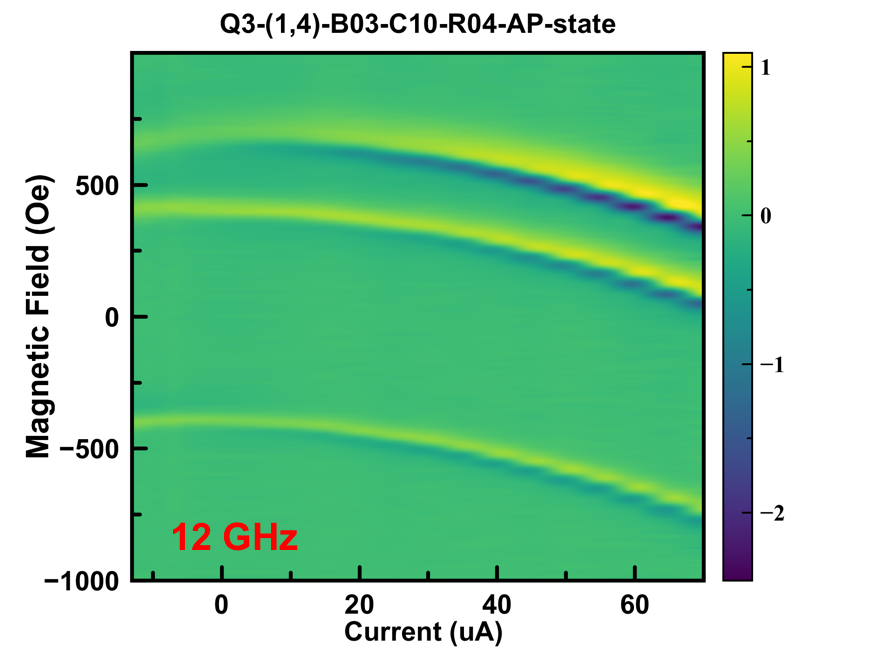
\includegraphics[width=75mm]{fig/2018/C10DC}}
\subfigure{\label{fig:C10DCamp}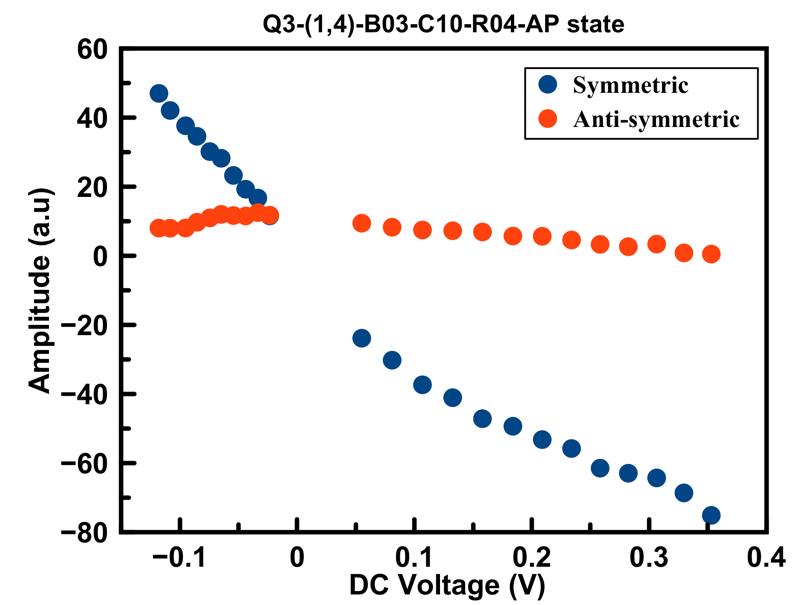
\includegraphics[width=75mm]{fig/2018/C10DCsignal}}
\caption{(a) The bias-dependent ST-FMR field sweep spectrum at AP state with 12 GHz. (b) FMR signal amplitude versus applied dc voltage. }
\end{figure}

After we vary the applied the power in the ST-FMR measurement, it is also interesting to change the dc bias. Fig.\ref{fig:C10DC} shows the bias-dependent ST-FMR field sweep spectrum at AP state with 12 GHz. All the three modes have the same curvature under external bias, which proves that these are all the spin-wave modes from the free layer. Fig.\ref{fig:C10DCamp} shows the FMR signal amplitude versus applied dc voltage. We find that the symmetric component(relating to spin transfer torque) shows a quadric+linear dependent and the anti-symmetric component was nearly invariant versus bias.

\begin{figure}[!ht]
  \centering
  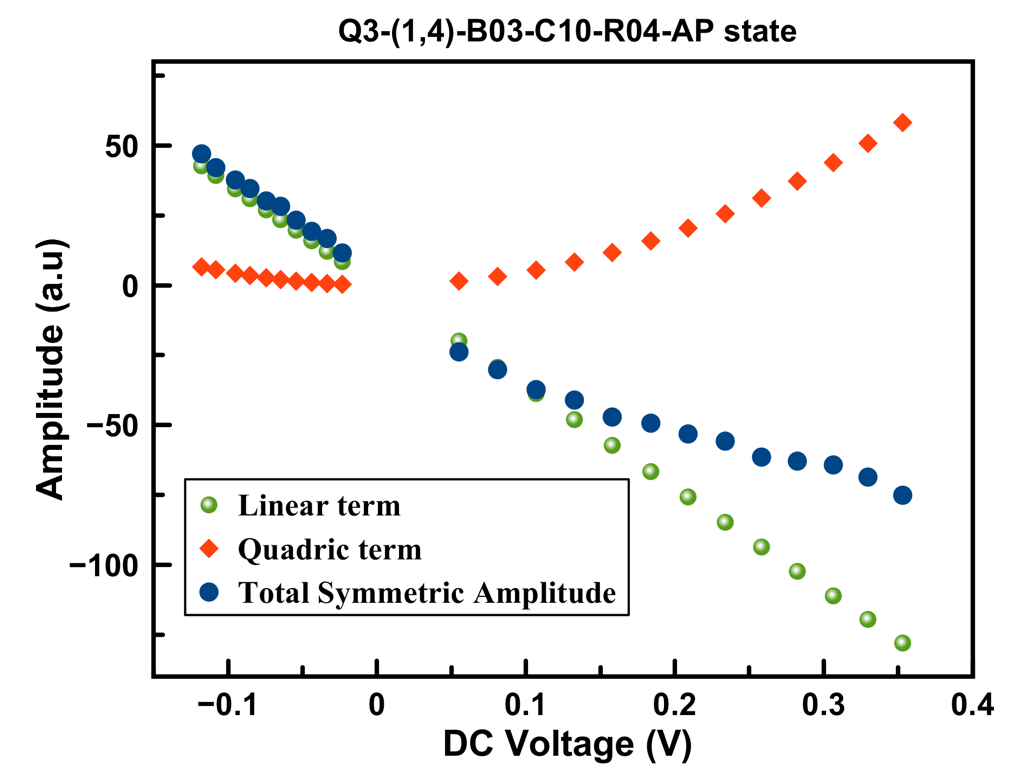
\includegraphics[width=0.6\textwidth]{fig/2018/C10DCFIT}
   \caption{Fitting of the FMR symmetric amplitude versus DC voltage as a sum of linear term and quadric term.}
  \label{fig:C10DCfit}
\end{figure}

We can further analyze the FMR symmetric amplitude versus DC voltage as shown in Fig.\ref{fig:C10DCfit}. The Symmetric amplitude shows as sum of linear term and quadric term. The linear term, related to the photo-resistance contribution, changes the sign with different polarity of dc voltage. Moreover, the linear term is nearly dominated except at large dc voltage, which indicating that the photo-resistance effect is not negligible in the system!

\begin{figure}[!ht]
  \centering
  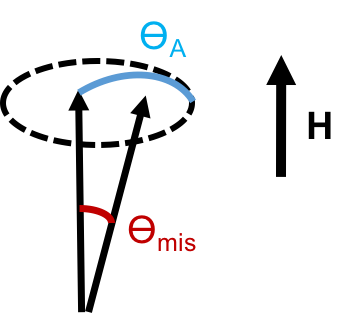
\includegraphics[width=0.4\textwidth]{fig/2018/demo}
   \caption{Demo of Perpendicular magnetized MTJs angle oscillation with out-of-plane magnetic field.}
  \label{fig:demo}
\end{figure}

The ST-FMR signal of MTJs with PMA can be modeled as shown in the Fig.\ref{fig:demo}. In the MTJs, there is a small angle $\theta_{mis}$ between the free layer and the fixed layer. The magnetic field H is applied in the perpendicular direction. After apply dc bias and microwave power, the resistance of the MTJ can be written as 
	\begin{equation}
		R = R_{dc} + R_{ac} \sin{\omega t} + R_{20} \sin{2 \omega t} 
	\end{equation}
	
Here the $R_dc$ is the time-averaged MTJ resistance and $R_ac$ is the oscillating MTJ resistance. $R_{20}$ is the higher harmonic component of the resistance. The amplitude the angular oscillation is $\theta_A$. After we define those variables, the ST-FMR signal can be expressed as 
\begin{equation}
	V_{ST-FMR} \propto I_{dc}R_{dc} + \frac{1}{2} <I_{ac}R_{ac}>
\end{equation}

The first term is related with contributions from photo-voltage(related to rectification) and the second term is related with photo-resistance(related to time-averaged resistance).


\begin{figure}[!ht]
\centering
\subfigure{\label{fig:C10DCFH}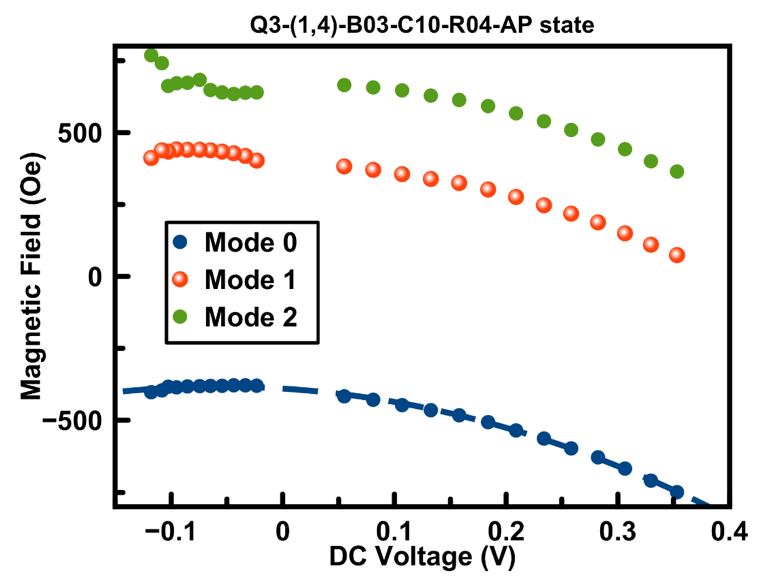
\includegraphics[width=75mm]{fig/2018/C10DC-FH}}
\subfigure{\label{fig:C10DCLW}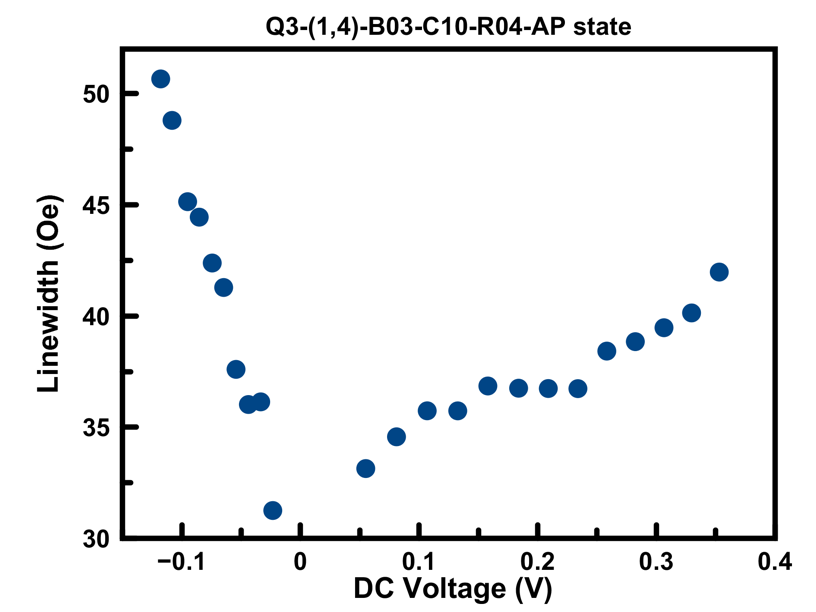
\includegraphics[width=75mm]{fig/2018/C10DC-LW}}
\caption{(a) The resonance field versus bias for three modes. (b) Mode 0 HWHM linewidth versus applied dc bias.}
\end{figure}

Before we end this section, we can also fit the spin-wave modes under finite dc bias. Fig.\ref{fig:C10DCFH} shows the resonance field versus bias for three modes. The main mode has both linear and quadratic dependence. The quadratic dependence is harder to analyze since it is a mixed contribution from field-like torque and ohmic heating. The linear term is believed to relate with voltage-controlled magnetic anisotropy(VCMA). The linear slope gives VCMA 244 Oe/V, close to previously measured circular devices. Fig.\ref{fig:C10DCLW} shows Mode 0 HWHM linewidth versus applied bias. At positive voltage(damping), we find the linewidth increase as increasing voltage(as expected). At negative voltage(anti-damping),however, the linewidth unexpectedly increase with larger negative voltage. This is also a strong evidence of non-linear damping in this type of devices. One possible explanation is that, when approaching the switching region, the free layer has more fluctuations which contributes to the linewidth broadening.







\clearpage




\section{Summary of Circular Devices: Experimental Data}

Now we would like to summarize the experimental data of circular devices with different diameters. As we have demonstrated in Fig.\ref{fig:C07FH}, the signature of the spin wave modes excited in these devices are one lowest quasi-uniform main mode(Mode 0) with two split higher-order modes(Mode 1 Mode 2). For each dimension, we can measure over ten devices to obtain mode statistics. The idea of measuring nominally identical devices is to reduce random sample-to-sample variations. For each measured device, we can list the frequencies of three spin-wave modes at zero magnetic field. These raw data can be found from the appendix. From the mode statistics we can extract the average mode frequency and standard deviations.

\begin{figure}[!ht]
  \centering
  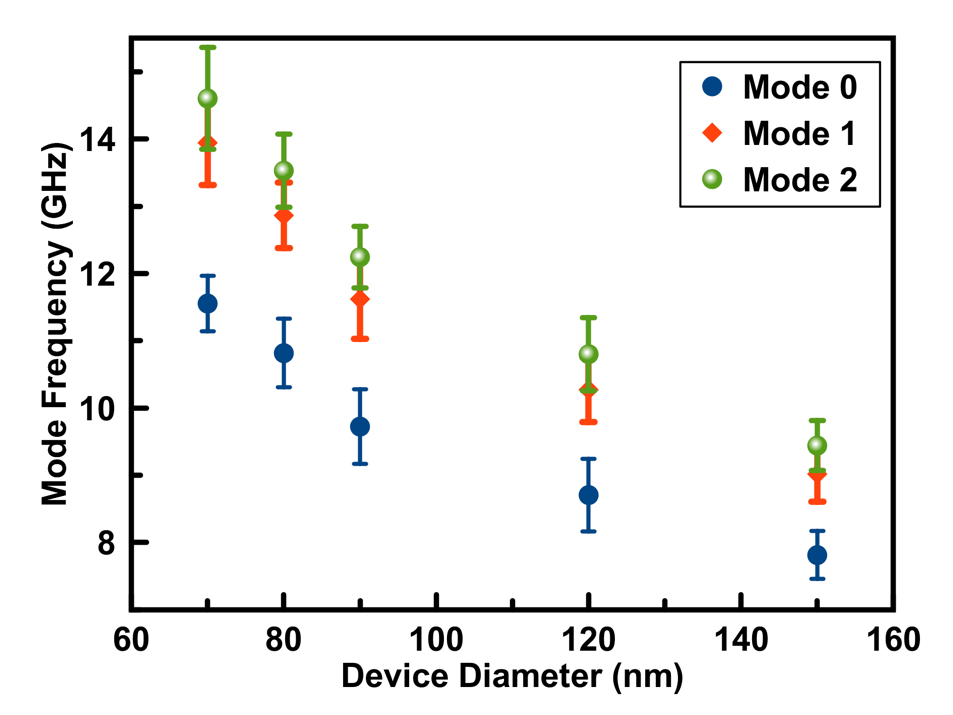
\includegraphics[width=0.6\textwidth]{fig/2018/ModevsSize}
   \caption{Summary of main mode of all the three modes. The error bar indicates the standard deviations obtained from sample statistics.}
  \label{fig:ModeVsSize}
\end{figure}

The summary of main mode and standard deviations of all the three modes are plotted in Fig.\ref{fig:ModeVsSize}. As the device diameter goes up, the mode frequencies of three modes reduces due to shape anisotropy reduction.

Now let us first focus on the main mode and plot it as a function of device diameter as shown in Fig.\ref{fig:GapvsSize}. The effective demagnetization factor is given by\cite{demagfactor}.

\begin{equation}\label{eq:Nz}
	\centering
	N_z \approx 1- \frac{1}{\pi d} [2 \ln(4 \frac{d}{t} ) -1 ]
\end{equation}

where the d is the device diameter and t is the free layer thickness. From Eq.\ref{eq:Nz} and the fact that $N_x + N_y + N_z = 1$, the total perpendicular anisotropy $H_{ku}$ can be written as\cite{Kittel}

\begin{equation}\label{eq:Hk}
	\centering
	H_k = H_{ku} + 2 \pi (1 - 3 N_z) M_s
\end{equation}

Assuming the free layer thickness 1.6 nm, the fitted result  $M_s \ 1820 \ \text{emu}/cm^3$ and  $H_{ku} \ 24 \ \text{KOe}$, which is comparably with other independent measured values.

\begin{figure}[!ht]
\centering
\subfigure{\label{fig:GapvsSize}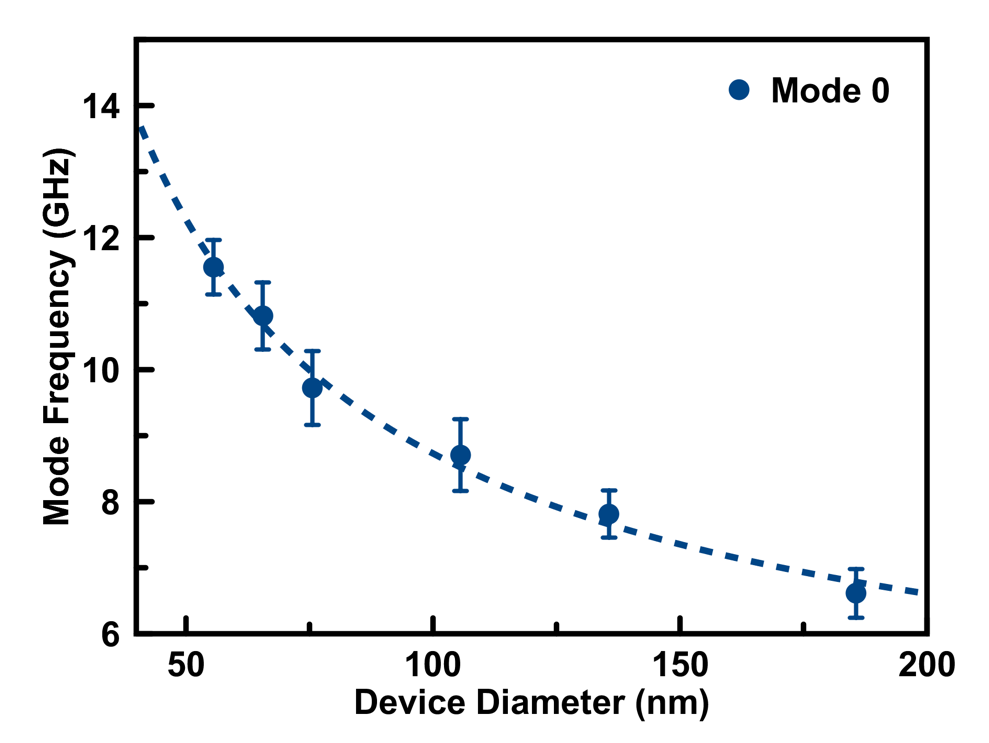
\includegraphics[width=75mm]{fig/2018/GapvsSize}}
\subfigure{\label{fig:LinearFit}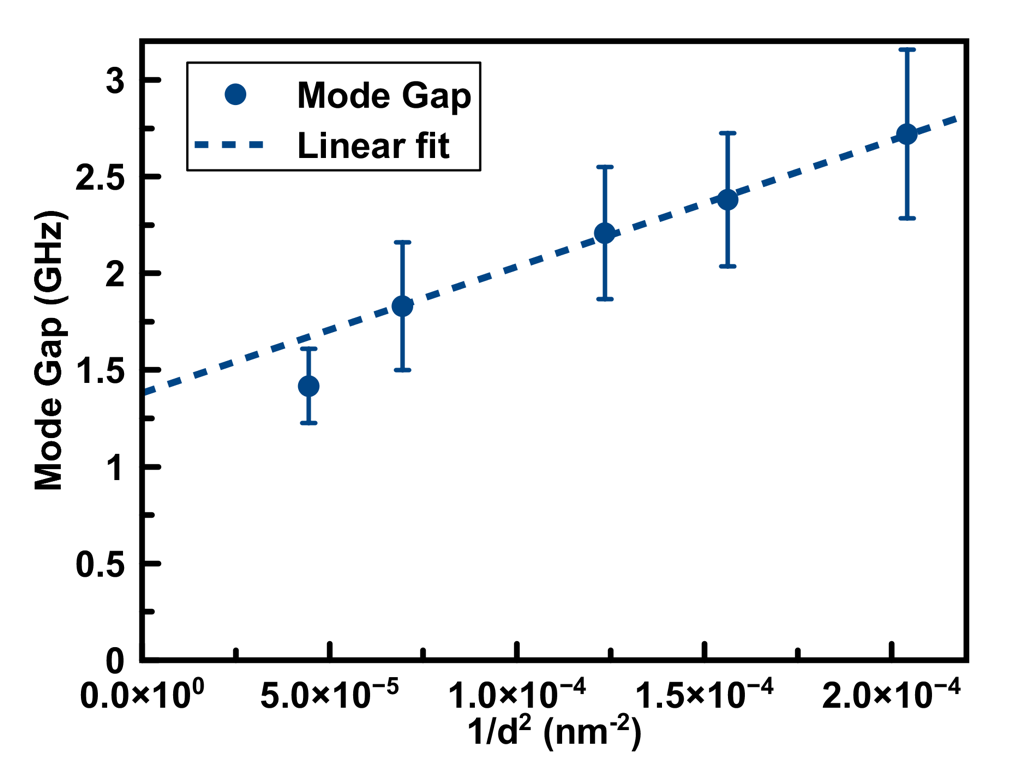
\includegraphics[width=75mm]{fig/2018/LinearFit}}
\caption{(a) Main mode frequency is plotted as a function of 
device diameter. (b) Mode Gap plotted as a function $1/d^2$ with d represents the diameter of the device.}
\end{figure}



Fig.\ref{fig:LinearFit} shows mode gap plotted as a function $1/d^2$ with d represents the diameter of the device. The mode gap between first two modes in a circular device can be modeled as
\begin{equation}
	\hbar (\omega_1 - \omega_0 ) = D (s/d)^2
\end{equation}

Here $\omega = 2\pi  f$ represents the frequency of the mode. D is the exchange stiffness which is related with exchange constant $Aex$ by $A_{ex} = \frac{D M_s}{2 g \mu_B} $. (g: g-factor. $M_s$ saturation magnetization. $\mu_B$ Bohr magneton). s is a numerical factor which is close to 3.68. By perform a linear fit of Fig.\ref{fig:LinearFit} we can obtain the $A_{ex}$ value of 8.9 pJ/m, which is reduced from the bulk value around 15 pJ/m.

\clearpage


\section{Micromagnetic Simulations of the Mode Spacing}

\begin{figure}[!ht]
  \centering
  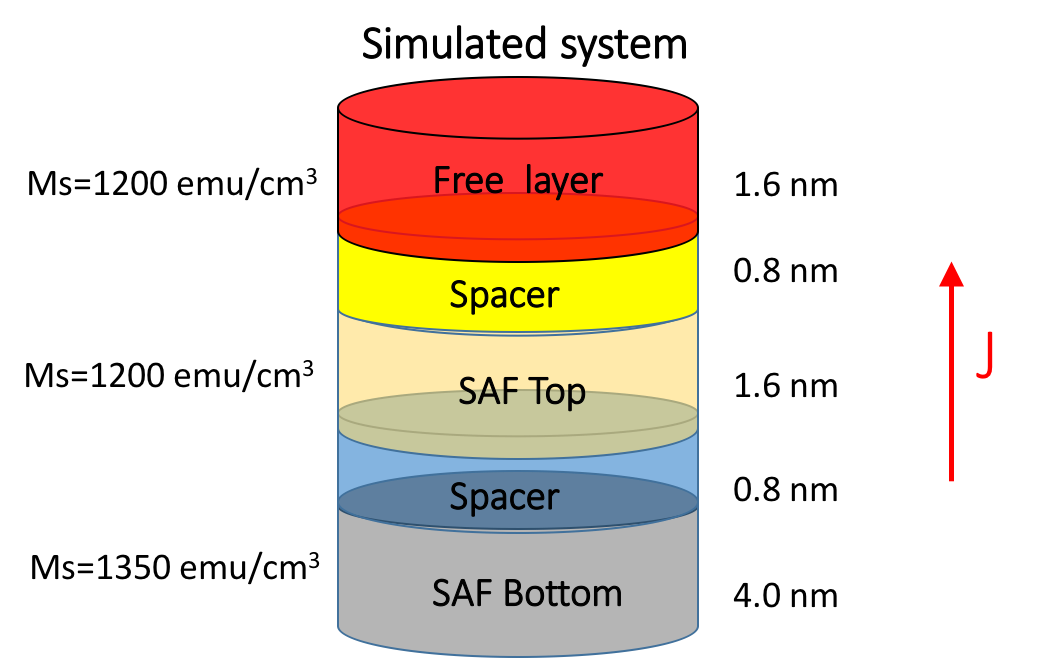
\includegraphics[width=0.8\textwidth]{fig/2018/simulated}
   \caption{Simulated MTJ System}
  \label{fig:simulated}
\end{figure}



Used parameter $ A_ex  12 pJ/m $
$ K_u 10.5*105 J/m^3$


\begin{figure}[!ht]
\centering
\subfigure{\label{fig:7070}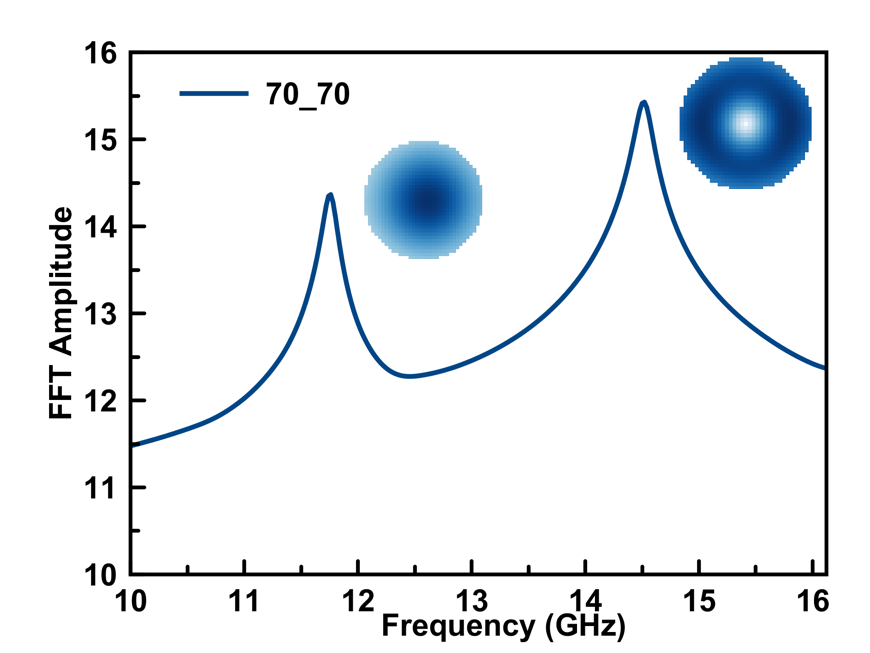
\includegraphics[width=50mm]{fig/2018/sim/70_70}}
\subfigure{\label{fig:ellipse}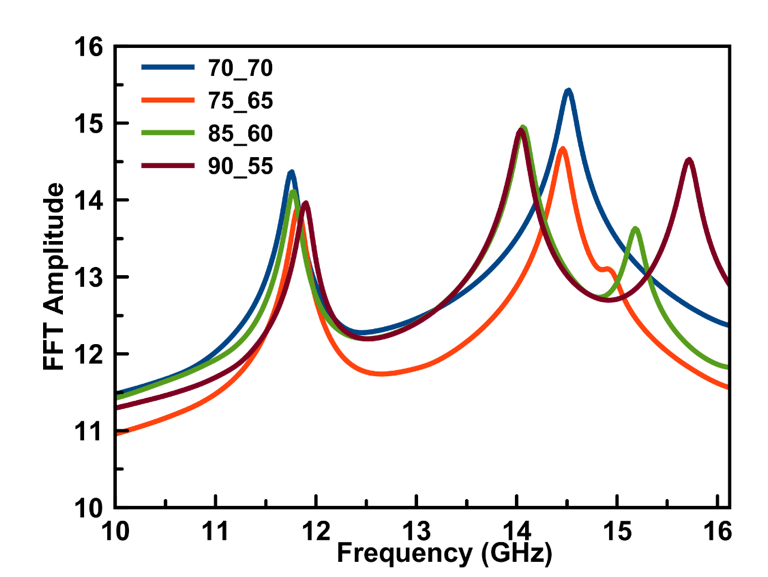
\includegraphics[width=50mm]{fig/2018/sim/ellipse}}
\subfigure{\label{fig:shape}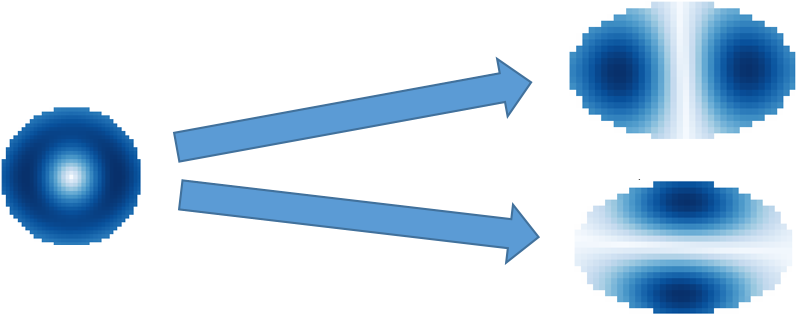
\includegraphics[width=50mm]{fig/2018/sim/split}}
\caption{}
\end{figure}



\begin{table}[ht!]
\centering
\begin{tabular}{|l|l|l|l|l|l|}
\hline
\textbf{} & \textbf{70*70} & \textbf{75*65} & \textbf{85*60} & \textbf{90*55} & \textbf{Experimental} \\ \hline
\textbf{Mode 0} & 11.74 & 11.82 & 11.78 & 11.9 & 11.55 \\ \hline
\textbf{Mode 1} & 14.5 & 14.46 & 14.06 & 14.04 & 13.94 \\ \hline
\textbf{Mode 2} &  & 14.9 & 15.2 & 15.72 & 14.6 \\ \hline
\textbf{Gap (1+2)/2-0} & 2.76 & 2.86 & 2.85 & 2.9 & 2.72 \\ \hline
\textbf{Gap 2-1} & 0 & 0.44 & 1.14 & 1.68 & 0.66 \\ \hline
\textbf{Aspect ratio} & 1 & 1.15 & 1.41 & 1.63 &  \\ \hline
\end{tabular}
\caption{Shape distortion}
\label{shapedist}
\end{table}


\begin{figure}[!ht]
  \centering
  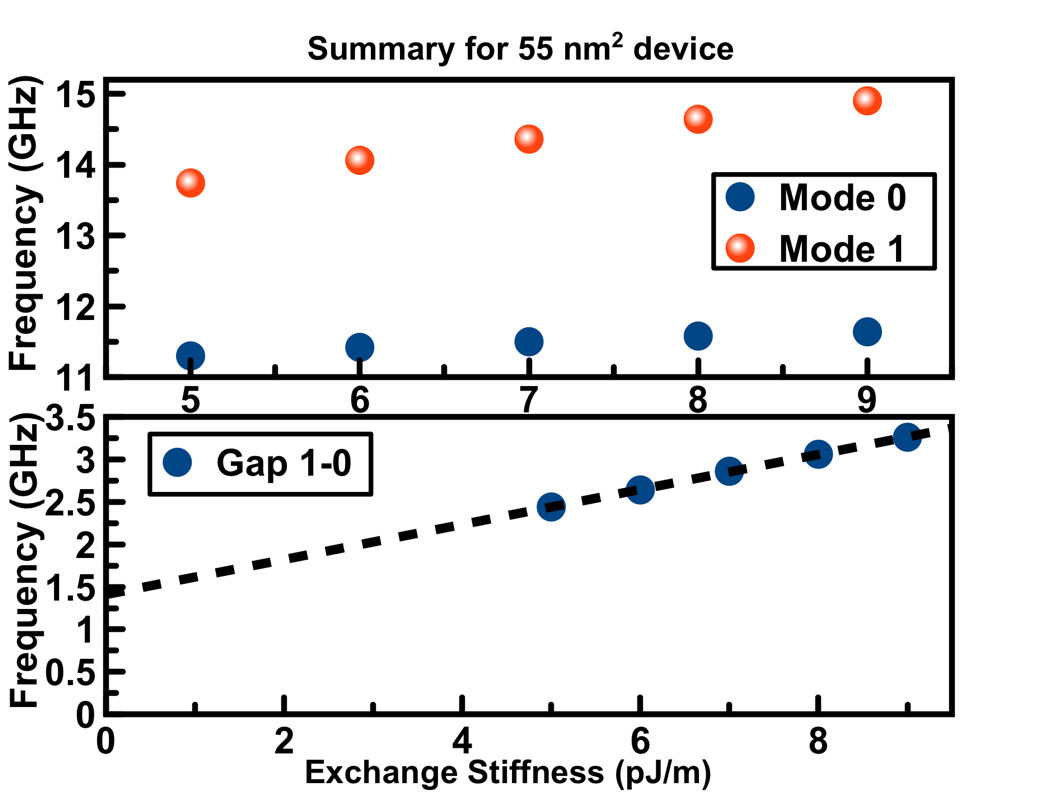
\includegraphics[width=0.8\textwidth]{fig/2018/sim/55sim}
   \caption{55 simulated}
  \label{fig:55sim}
\end{figure}



\begin{table}[ht!]
\centering
\begin{tabular}{ c c }
      \addheight{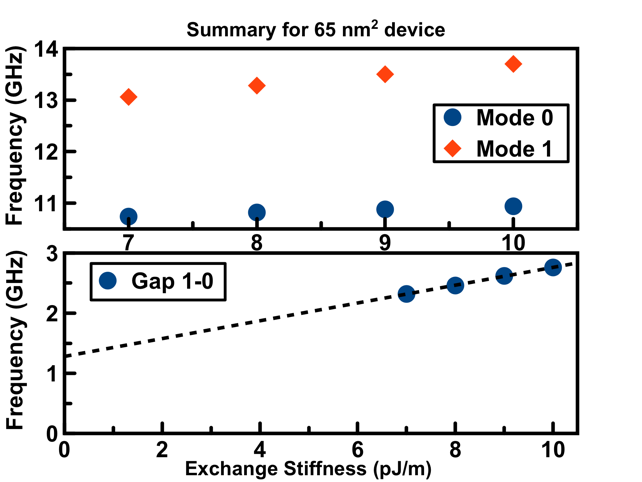
\includegraphics[width=60mm]{fig/2018/sim/65sim}} &
      \addheight{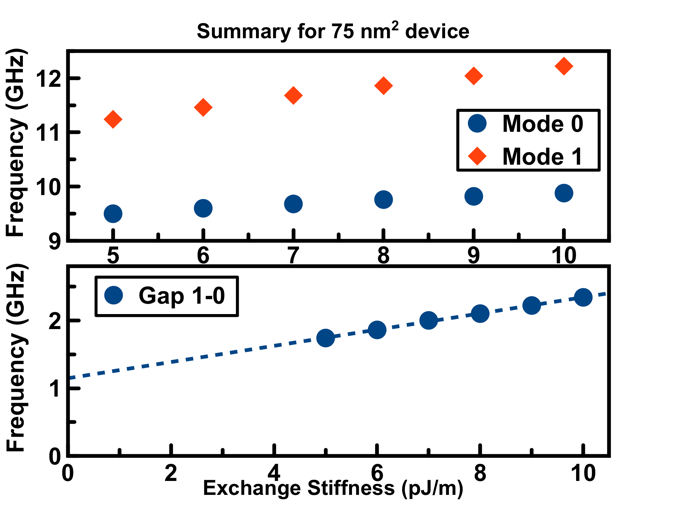
\includegraphics[width=60mm]{fig/2018/sim/75sim}} \\
      \addheight{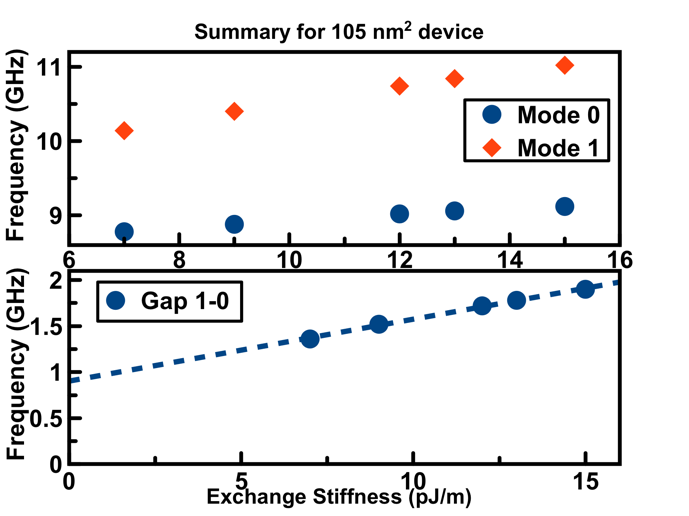
\includegraphics[width=60mm]{fig/2018/sim/105sim}} &
      \addheight{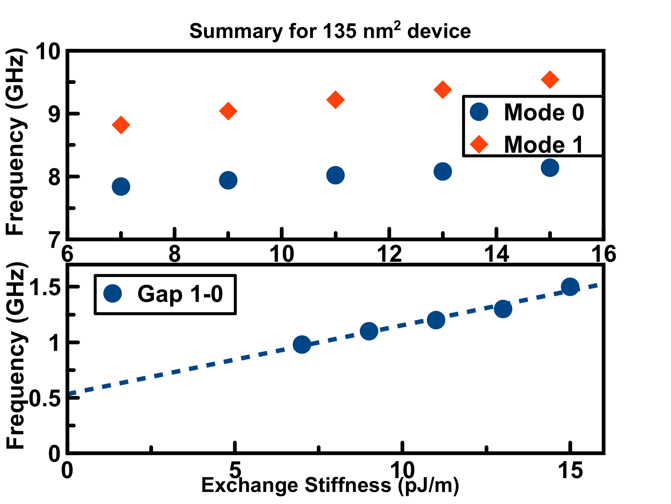
\includegraphics[width=60mm]{fig/2018/sim/135sim}} \\
\end{tabular}
\caption{Circular Device Simulation Summary}
\label{circularsummary}
\end{table}



\begin{figure}[!ht]
  \centering
  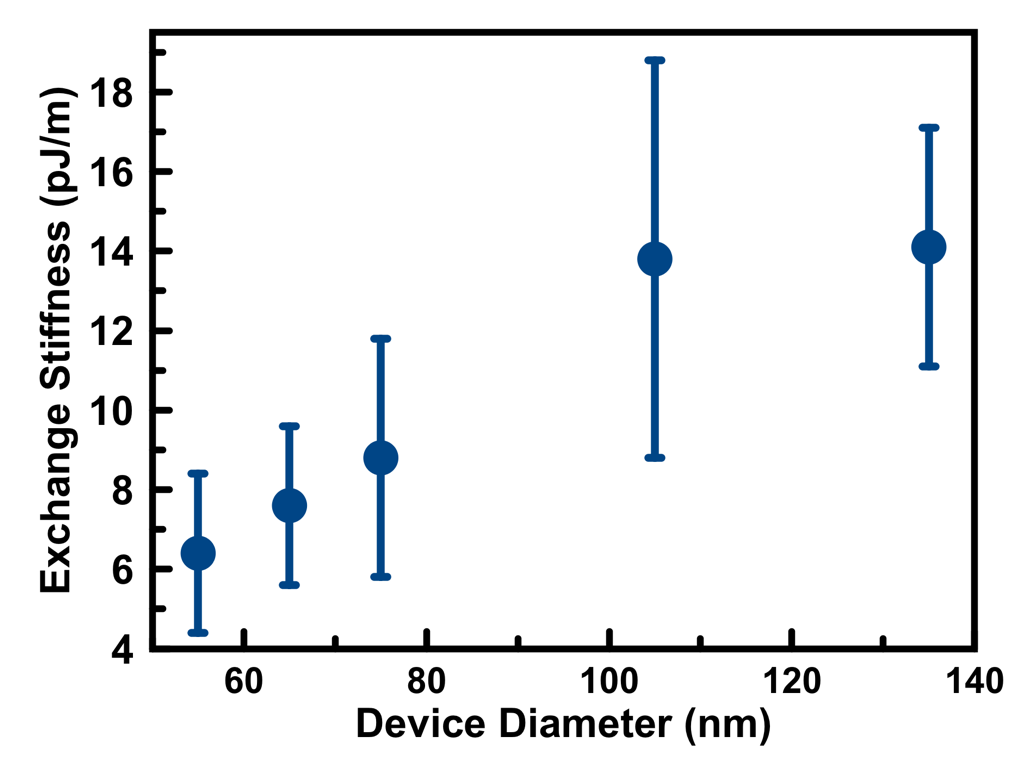
\includegraphics[width=0.6\textwidth]{fig/2018/sim/circular_summary}
   \caption{Circular Device Simulation Summary}
  \label{fig:circularsummary}
\end{figure}


\begin{table}[]
\centering
\begin{tabular}{|l|l|l|l|}
\hline
\textbf{Nominal Device length (nm)} & \textbf{Device Length* (nm)} & \textbf{Aex (pJ/m)} & \textbf{Error (pJ/m)} \\ \hline
\textbf{70} & 55 & 6.4 & 2 \\ \hline
\textbf{80} & 65 & 7.6 & 2 \\ \hline
\textbf{90} & 75 & 8.8 & 3 \\ \hline
\textbf{120} & 105 & 13.8 & 5 \\ \hline
\textbf{150} & 135 & 14.1 & 3 \\ \hline
\end{tabular}
\caption{Circular Device Fit Summary}
\label{cirexsummary}
\end{table}


\begin{figure}[!ht]
  \centering
  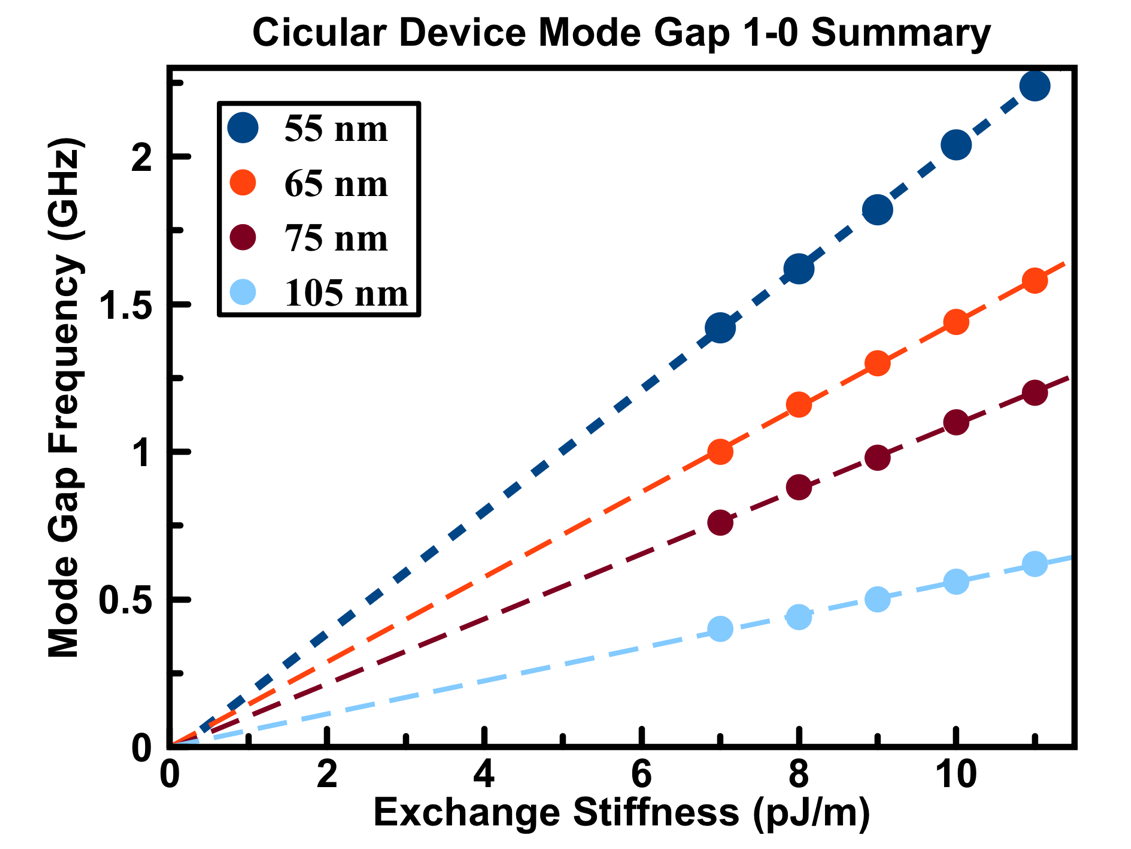
\includegraphics[width=0.6\textwidth]{fig/2018/sim/free_only_circular}
   \caption{Single Free layerCircular Device Simulation Summary}
  \label{fig:freecircularsummary}
\end{figure}



